\chapter{Polynomial time algorithms using price of connectivity}\label{chap2}

For some graph classes it has been shown that the numbers \(\tau_c\) and \(\tau\) differ on by an additive constant.
Similar results exist for graph parameters different from \(\tau\).
Chiarelli, Hartinger, Johnson, Milanič, Paulusma in \cite{ChiarelliHartinger18} present a general technique that utilizes a constant difference between \(\tau_c\)
and \(\tau\).
to design polynomial time algorithms. 

\begin{lemma}[\citet{ChiarelliHartinger18}]\label{algo:polylemma}
	Let \(\pi\) be a property of a set of vertices, which if it holds for a set \(S\) then it holds for every superset.
	Suppose that for every \(G\) from a class \(\mathcal{G}\) all minimal vertex sets satisfying the property \(\pi\) can be enumerated in polynomial time.
	Also the size of a minimum connected set of vertices with the property \(\pi\) is at most \(\pi(G) + c\) for a constant \(c\). 
	Then a minimum connected vertex set with the property \(\pi\) can be found in polynomial time for every \(G \in \mathcal{G}\).
\end{lemma}
The vertex cover and the dominating set are examples of graph properties closed under supersets on the other hand independent set is an example of a property which is not. 

\begin{myproof}
	The algorithm works as follows. Enumerate all minimal vertex sets with property \(\pi\). 
	For each minimal set consider all possibilities of adding at most \(c\) vertices and check 
	if the new set is connected.
	The smallest connected set of vertices found is returned.
	Notice that this algorithm is polynomial.
	
	Suppose that a set \(S\) is a minimum connected set with property \(\pi\).
	We need to show that the algorithm will return \(S\) or another minimum set with the same size.
	Pick from \(S\) a minimal set with property \(\pi\) and denote it by \(S'\).
	The set \(S'\) will be one of the enumerated sets by definition. Due to the facts that \(|S| \leq {\pi(G) + c}\) and \(|S'| \geq \pi(G)\) we have \(|S| - |S'| \leq c\).
	Hence, \(S\) will be found.
\end{myproof}
We continue with demonstration of making use of Lemma~\ref{algo:polylemma} to create polynomial algorithms for connected vertex cover and
connected feedback vertex set following ideas from \cite{ChiarelliHartinger18}.
In this part we focus on a class of \(sP_2\)-free graphs, where \(sP_2\) denotes a disjoint union of \(s\) paths on two vertices.
(See Figure \ref{f4}.)
\begin{figure}
\centering
\begin{minipage}{.45\textwidth}
  \centering
  \begin{tikzpicture}
        \tikzstyle{vertex} = [circle, minimum width=4pt, draw, inner sep=0pt, fill=white]

        \foreach \i in {1,...,3}
        {
                \node[vertex] (u\i) at ($(0,0) + (0, \i)$) {};
                \node[vertex] (v\i) at ($(1,0) + (0, \i)$) {};
                \draw (u\i)--(v\i);
        }
\end{tikzpicture}


  \caption*{\(3P_2\)}
\end{minipage}%
\begin{minipage}{.5\textwidth}
  \centering
  \begin{tikzpicture}
        \tikzstyle{vertex} = [circle, minimum width=4pt, draw, inner sep=0pt, fill=white]
        \foreach \i in {1,...,3}
        {
                \node[vertex] (u\i) at ($(0,0) + (0, \i)$) {};
                \node[vertex] (v\i) at ($(1,0) + (0, \i)$) {};
                \draw [red] (u\i) -- (v\i);
                \ifnum \i > 1
                        \begin{scope}[on background layer]
                        \draw (u\i) -- ($(u\i) + (0, -1)$);
                        \draw (v\i) -- ($(v\i) + (0, -1)$);
                        \end{scope}
                \fi

                \ifnum \i=2
                   \node[vertex] (a) at ($(v\i) + (1, 0)$) {};
                   \node[vertex] (b) at ($(v\i) + (2, 0)$) {};
                   \draw (a)--(v\i);
                   \draw [red] (a)--(b);
                        \draw (u\i)--(v\i);
                        
                \fi
        
        }
\end{tikzpicture}


  \caption*{Graph with induced \(3P_2\)}
\end{minipage}
\begin{minipage}{.45\textwidth}
  \centering
  \begin{tikzpicture}
        \tikzstyle{vertex} = [circle, minimum width=4pt, draw, inner sep=0pt, fill=white]
%%
        \foreach \i in {1,...,3}
        {
                \node[vertex] (u\i) at ($(0,0) + (0, \i)$) {};
                \node[vertex] (v\i) at ($(1,0) + (0, \i)$) {};
                \draw (u\i) -- (v\i);
                \ifnum \i > 1
                        \begin{scope}[on background layer]
                        \draw (u\i) -- ($(u\i) + (0, -1)$);
                        \draw (v\i) -- ($(v\i) + (0, -1)$);
                        \end{scope}
                \fi

                \ifnum \i=2
                   \node[vertex] (a) at ($(v\i) + (1, 0)$) {};
                   \node[vertex] (b) at ($(v\i) + (2, 0)$) {};
                   \draw (a)--(v\i);
                   \draw (a)--(b);
                   \draw (v1)--(a);
                   \draw (v3)--(a);

                \fi

        }
\end{tikzpicture}


  \caption*{\(3P_3\)-free graph}
\end{minipage}
  \caption{Examples illustrating \(3P_2\)-free graphs.}
  \label{f4}
\end{figure}

\begin{thm}[\citet{BalasYu89}]\label{algo:1}
For every constant \(s \geq 1\), the number of maximal independent sets
of an \(sP_2\)-free graph on \(n\) vertices is at most \(n^{2s} + 1\).
\end{thm}

\begin{thm}[\citet{TsukiyamaIde77}]\label{algo:2}
For every constant \(s \geq 1\), it is possible to enumerate all maximal
independent sets of a graph \(G\) on \(n\) vertices and \(m\) edges with a delay of \(O(nm)\).
The delay is defined here as the maximal number of steps before the first and between any two consecutive outputs.
\end{thm}

Recall that vertices not included in a maximal independent set belong to a minimal vertex cover.
Both theorems together imply, that it is possible to enumerate all minimal vertex covers in \(sP_2\)-free graphs in polynomial time.
To fulfill all assumptions of Lemma~\ref{algo:polylemma} we need to show, that the numbers \(\tau\) and \(\tau_c\) differ only by an additive constant.

\begin{thm}[\citet{HartingerPaulusma16}]\label{algo:3}
Let \(s \geq 1\) and let \(G\) be a connected \(sP_3\)-free graph.  
Then the size of a minimum connected vertex cover of \(G\) is at most \(\tau + 4s^{2} + 2s - 10\).
\end{thm}

Theorems \ref{algo:1}, \ref{algo:2}, \ref{algo:3} and Lemma~\ref{algo:polylemma} 
imply the following theorem.

\begin{thm}[\citet{ChiarelliHartinger18}]\label{algo:4}
For every constant \(s \geq 1\) a minimum connected vertex cover can be found
in polynomial time in \(sP_2\)-free graphs.
\end{thm}

In the same fashion as before we will use Lemma~\ref{algo:polylemma} to design an algorithm for the minimum connected feedback vertex set.
\begin{defn}[Feedback vertex set]
A set of vertices \(S\) is called a \emph{feedback vertex set} if the graph \(G\setminus S\) does not contain any cycles.
\end{defn}

\begin{thm}[\citet{ChiarelliHartinger18}]\label{algo:sp2feedback}
Minimum connected feedback vertex set is polynomial time solvable for a class of \(sP_2\)-free graphs.
\end{thm}

\begin{thm}[\citet{BelmonteHofKaminskiPaulusma17}]\label{algo:5}
Let \(s \geq 1\) and let \(G\) be a connected \(P_3\)-free graph. 
Let \(f\) be the size of a minimum feedback vertex set of \(G\). 
Then the size of a minimum connected feedback vertex set of \(G\) is at most \(f + 12s^2 - 2s - 2\).
\end{thm}

\begin{thm}[\citet{SchwikowskiSpeckenmeyer10}]\label{algo:feedbackdelay}
It is possible to enumerate all minimal feedback vertex sets of a
graph \(G\) on \(n\) vertices and \(m\) edges with a delay of \(O(n^3 + n^2 m)\).
Delay is defined the same as in Theorem~\ref{algo:2}.
\end{thm}

\begin{lemma}[\citet{ChiarelliHartinger18}]\label{algo:feedbackpoly}
	For every \(s \geq 1\) exists a constant \(c_s\) such that number of minimal feedback vertex sets in any \(sP_2\)-free graph on \(n\) vertices is \(O(n^{c_s})\).
\end{lemma}

\begin{myproof}
	Let \(S\) denote the minimal feedback vertex of a graph \(G\).
	The complementary graph \(G - S\) is a forest \(F_S\).
	We define a \emph{skeleton} \(F_S'\) of a forest \(F_S\) as the following subgraph. 
	From the components of \(F_S\) isomorphic to \(P_2\), we delete an arbitrary vertex; from the remaining components delete all leaves. 
	We observe that the set of vertices \(l(F'_S) := V(F_S) \setminus V(F'_S)\) is an independent set in \(G\) and each vertex has at most one neighbor in \(F'_S\).
	(See Figure~\ref{fig:fsprime} with an example.)
	Let \(J(F'_S)\) be a subset of vertices \(V(G) \setminus V(F'_S)\) which have at most one neighbor in \(F'_S\).
	\begin{claim}
		The set \(l(F'_S)\) is a maximal independent set of \(G[J(F'_S)]\).
	\end{claim}
	To prove the claim suppose that in \(J(F'_S) \setminus l(F'_S)\) there exists a vertex \(v\) non-adjacent to vertices in \(l(F'_S)\). 
	Then \(G[F_S \cup \{v\}]\) is a forest; thus, \(S \setminus \{v\} \) is also a feedback vertex set. That contradicts the minimality of \(S\).
	In other words, the set \(J(F'_S)\) consists only of \(l(F'_S)\) and vertices from \(S\). The claim is proved.

	To find all minimal feedback vertex sets in a given graph \(G\), 
	we consider every skeleton and check every maximal independent set on the rest of the vertices incident to at most one vertex of the skeleton.
	Next we test whether the vertices neither included in the skeleton nor the maximal independent set are minimal feedback vertex set of \(G\).
	The number of all maximal independent sets is upper-bounded by the expression \(n^{2s} + 1\) according to Theorem~\ref{algo:1}. 
	To complete the proof it suffices to show that the number of all skeletons is polynomial in \(n\), 
	because  that the number of minimal feedback vertex sets is also polynomial in \(n\).
	
	\begin{claim}
		\(|V(F'_S)| \leq 3s^2 - 5s + 2.\)
	\end{claim}
	One way how to estimate the number of vertices in a forest \(F'_S\) 
	is to decompose each component \(C\) into paths going from its leaves to a fixed vertex. 
	These paths contain all vertices in \(C\), eventhough some vertices can be counted multiple times.
	Roughly speaking, using the assumption that \(G\) is \(sP_2\)-free, we show that number of leaves is at most \(s - 1\) 
	and the length of the longest path in \(C\) is at most \(3s - 2\). 
	The latter is true for any induced path of \(G\), as path on \(3s - 1\) vertices contains \(s\) disjoint copies of \(P_2\).
	Let us define and estimate the number of leaves. 
	Set \(A\) of vertices of \(F'_S\) contains all isolated vertices of \(F_S'\), 
	from each component isomorphic to \(P_2\) one arbitrary vertex and lastly from the rest of the components all vertices of degree \(1\).
	Each vertex from \(A\) has at least one neighbor in \(l(F'_S)\) by definition of \(F'_S\), for each vertex we pick one such neighbor.
	These pairs induced disjoint set of \(P_2\). Number of these pairs is at most \(s - 1\).
	Now consider paths from vertices in \(A\) to a fixed vertex in the same component. 
	This concludes the proof of the claim. 

	The number of all possible choices of a skeleton is \(O(n^{3s^2})\) and the number of all choices for a maximal independent set is \(O(n^{2s})\).
	Therefore, there is a constant \(c_s\) depending on \(s\) such that the number of all minimal feedback vertex sets in \(G\) is \(O(n^{c_s})\).
\end{myproof}

\begin{proof}[Proof of Theorem~\ref{algo:sp2feedback}]
The previous lemma and Theorem~\ref{algo:feedbackdelay} 
imply that the minimum feedback vertex set can be found in polynomial time by enumerating all minimal feedback vertex sets in \(sP_2\)-free graphs.
The property of being a feedback vertex set holds for supersets. 
By Theorem~\ref{algo:5} the difference between both parameters is constant.
All assumptions of Lemma~\ref{algo:polylemma} are satisfied, so there is an algorithm that finds a minimum connected feedback vertex in polynomial time in \(sP_2\)-free~graphs.
\end{proof}

\begin{figure}
\centering
\begin{minipage}{.45\textwidth}
	\centering
	     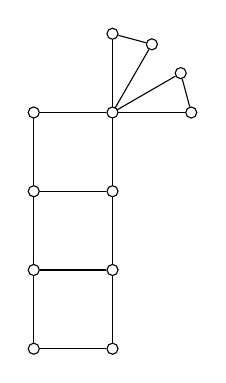
\begin{tikzpicture}

                \tikzstyle{vertex}  = [circle, minimum width=4pt, draw, inner sep=0pt, fill=white]
                \begin{scope}[shift={(1,3)}]

                \newdimen\R
                \R=1cm
                        \foreach \x in {0, 30, 60, 90}
                       {
                        \node [vertex](w\x) at (\x:\R) {};
                        \draw (0,0) -- (w\x);
                       }

                        \draw (w0) -- (w30);
                        \draw (w60) -- (w90);
                \end{scope}

                \foreach \x in {0, 1,...,3}
                {
                        \node [vertex](v\x) at (0, \x) {};
                        \node [vertex](u\x) at (1, \x) {};
                        \ifnum \x<3
                                \draw (v\x) -- ++(0,1);
                                \draw (u\x) -- ++(0,1);
                        \fi

                        \draw (u\x) -- (v\x);

                }

        \end{tikzpicture}



	\caption*{\(5P_2\)-free graph \(G\).}
	%%\label{fig:fex}
\end{minipage}
\begin{minipage}{.45\textwidth}
	\centering
	\begin{tikzpicture}

                \tikzstyle{vertex}  = [circle, minimum width=4pt, draw, inner sep=0pt, fill=white]
                \begin{scope}[shift={(1,3)}]

                \newdimen\R
                \R=1cm
                        \foreach \x in {0, 30, 60, 90}
                       {
                        \node [vertex](w\x) at (\x:\R) {};
                       }

                        \fill [red] (w0) circle (1.8pt);
                        \fill [red] (w60) circle (1.8pt);

                        \draw (w0) -- (w30);
                        \draw (w60) -- (w90);
                \end{scope}

                \foreach \x in {0, 1,...,3}
                {

                        \ifnum \x<3
                                \node [vertex, fill=red](v\x) at (0, \x) {};
                                \draw (v\x) -- ++(0,1);
                        \else
                                \node [vertex](v\x) at (0, \x) {};

                        \fi

                        \ifnum \x=0
                                \node [vertex](u\x) at (1, \x) {};
                                \draw (u\x) -- (v\x);
                        \fi

                        \ifnum \x=2
                                \node [vertex](u\x) at (1, \x) {};
                                \draw (u\x) -- (v\x);
                        \fi

                }
        \end{tikzpicture}


	\caption*{Set \(F_S\) and set \(F'_S\) in red.}
	%%\label{fig:fsprime}
\end{minipage}
\begin{minipage}{.45\textwidth}
	\centering
	     \begin{tikzpicture}

                \tikzstyle{vertex}  = [circle, minimum width=4pt, draw, inner sep=0pt, fill=white]
                \begin{scope}[shift={(1,3)}]

                \newdimen\R
                \R=1cm
                        \foreach \x in {0, 30, 60, 90}
                       {
                        \node [vertex](w\x) at (\x:\R) {};
                       }

                        \fill [red] (w0) circle (1.8pt);
                        \fill [red] (w60) circle (1.8pt);

                        \draw (w0) -- (w30);
                        \draw (w60) -- (w90);
                \end{scope}

                \foreach \x in {0, 1,...,3}
                {

                        \ifnum \x<3
                                \node [vertex](v\x) at (0, \x) {};
                                \draw (v\x) -- ++(0,1);
                        \else
                                \node [vertex](v\x) at (0, \x) {};

                        \fi

                        \ifnum \x=0
                                \node [vertex](u\x) at (1, \x) {};
                                \fill [red] (v\x) circle (1.8pt);

                                \draw (u\x) -- (v\x);
                        \fi

                        \ifnum \x=2
                                \node [vertex](u\x) at (1, \x) {};
                                \fill [red] (v\x) circle (1.8pt);
                                \draw (u\x) -- (v\x);
                        \fi

                }
                \end{tikzpicture}


	\caption*{Set \(A\) depicted in red.}
	%%\label{fig:fa}
\end{minipage}
	\caption{Illustration to the proof of Lemma~\ref{algo:feedbackpoly}.}
	\label{fig:fsprime}
\end{figure}

Using Lemma~\ref{algo:polylemma} directly fails 
if either the graphs have exponentially many minimal sets, or the difference between a minimal and a connected minimal set is no longer constant.

It is easy to construct connected \(2P_3\)-free graph with exponentially many maximal independent sets.
We will now show this construction. Let number of vertices be \(n = 3l + 1\).  
Divide \(3l\) vertices into \(l\) triples. The vertices in every triple induce a triangle. 
The remaining vertex \(v\) is set to be adjacent to every other vertex.
From each triple exactly one vertex can be added to the independent set, 
so the number of all maximal independent sets is \(3^{\frac{n-1}{3}}\).
Our graph is \(2P_3\)-free because every induced \(P_3\) needs to go through the central vertex \(v\).
Even though structural Theorems \ref{algo:3} and \ref{algo:5} still hold for \(sP_3\)-free graphs, we cannot assume 
that the number of minimal feedback vertex sets and maximal independent sets is polynomial in a number of vertices of \(G\).

Despite this fact there are still polynomial results for these problems using various techniques.
In the case of minimum size feedback vertex set \citet{Dabrowski20} constructed polynomial algorithm for \((sP_1 + P_3)\)-free and \(P_4\)-free graphs using structural properties of these classes.
For vertex cover, the authors of \cite{Grzesik19} use potential maximal cliques.
